%!TEX TS-program = xelatex
\documentclass[12pt, a4paper]{article}  

\usepackage{etex} % расширение классического tex в частности позволяет подгружать гораздо больше пакетов, чем мы и займёмся далее

%%%%%%%%%% Математика %%%%%%%%%%
\usepackage{amsmath,amsfonts,amssymb,amsthm,mathtools} 
%\mathtoolsset{showonlyrefs=true}  % Показывать номера только у тех формул, на которые есть \eqref{} в тексте.
%\usepackage{leqno} % Нумерация формул слева


%%%%%%%%%%%%%%%%%%%%%%%% Шрифты %%%%%%%%%%%%%%%%%%%%%%%%%%%%%%%%%
\usepackage{fontspec}         % пакет для подгрузки шрифтов
\setmainfont{Linux Libertine O}   % задаёт основной шрифт документа

\defaultfontfeatures{Mapping=tex-text}

% why do we need \newfontfamily:
% http://tex.stackexchange.com/questions/91507/
\newfontfamily{\cyrillicfonttt}{Linux Libertine O}
\newfontfamily{\cyrillicfont}{Linux Libertine O}
\newfontfamily{\cyrillicfontsf}{Linux Libertine O}

\usepackage{unicode-math}     % пакет для установки математического шрифта
\setmathfont{Asana Math}      % шрифт для математики

\usepackage{polyglossia}      % Пакет, который позволяет подгружать русские буквы
\setdefaultlanguage{russian}  % Основной язык документа
\setotherlanguage{english}    % Второстепенный язык документа


%%%%%%%%%% Работа с картинками %%%%%%%%%
\usepackage{graphicx}                  % Для вставки рисунков
\usepackage{graphics} 
\graphicspath{{images/}{pictures/}}    % можно указать папки с картинками
\usepackage{wrapfig}                   % Обтекание рисунков и таблиц текстом
\usepackage{subfigure}                 % для создания нескольких рисунков внутри одного
\usepackage{rotating}
\usepackage[export]{adjustbox}

%%%%%%%%%% Работа с таблицами %%%%%%%%%%
\usepackage{tabularx}            % новые типы колонок
\usepackage{tabulary}            % и ещё новые типы колонок
\usepackage{array}               % Дополнительная работа с таблицами
\usepackage{longtable}           % Длинные таблицы
\usepackage{multirow}            % Слияние строк в таблице
\usepackage{float}               % возможность позиционировать объекты в нужном месте 
\usepackage{booktabs}            % таблицы как в книгах!  
\renewcommand{\arraystretch}{1.3} % больше расстояние между строками





% Заголовок
\author{Решетникова Дарья} 
\title{Уютный факультатив по \LaTeX . Домашнее задание, номер 1.}
\date{\today}



\begin{document}

\begin{figure}[h!]
	\begin{minipage}[h!]{0.3\linewidth} 
		
	\begin{turn}{270}
		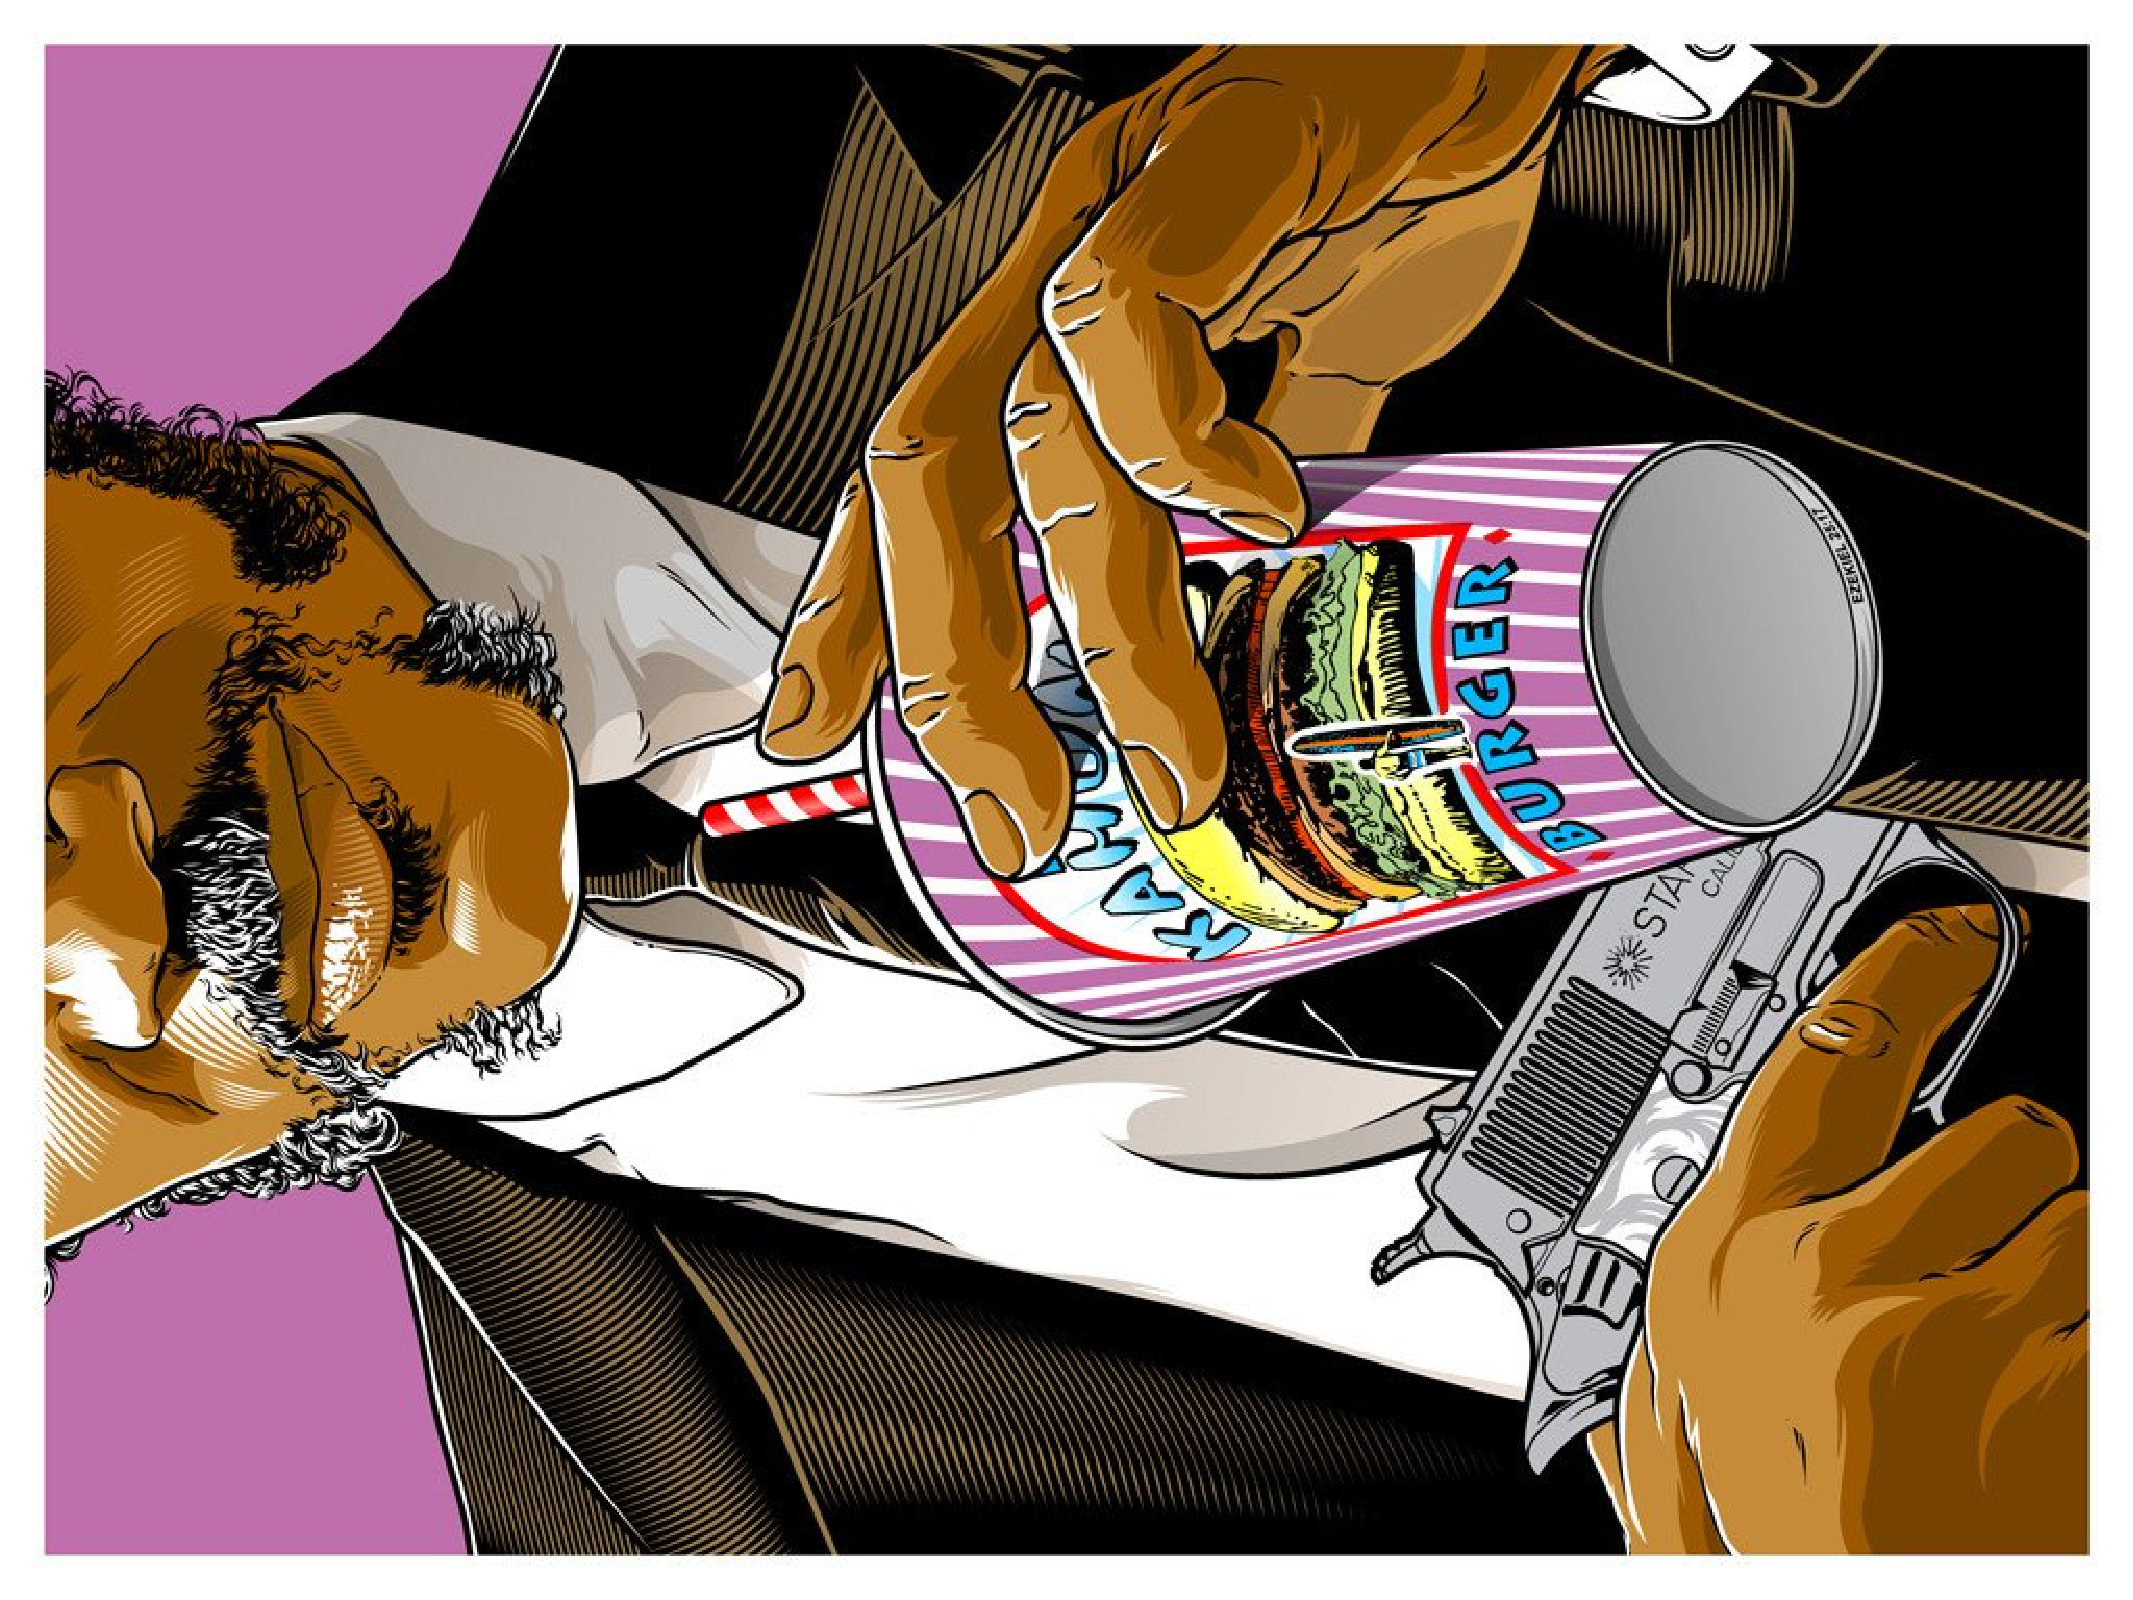
\includegraphics[height=5cm, width=6cm]{pop1.pdf}
	\end{turn}
	\end{minipage}
	\hfill
		\begin{minipage}[h!]{0.3\linewidth}
	 
\includegraphics[height=6cm, width=5cm]{pop3.pdf}
	\end{minipage}
\hfill
	\begin{minipage}[h!]{0.3\linewidth} 
	
	\begin{turn}{180}
		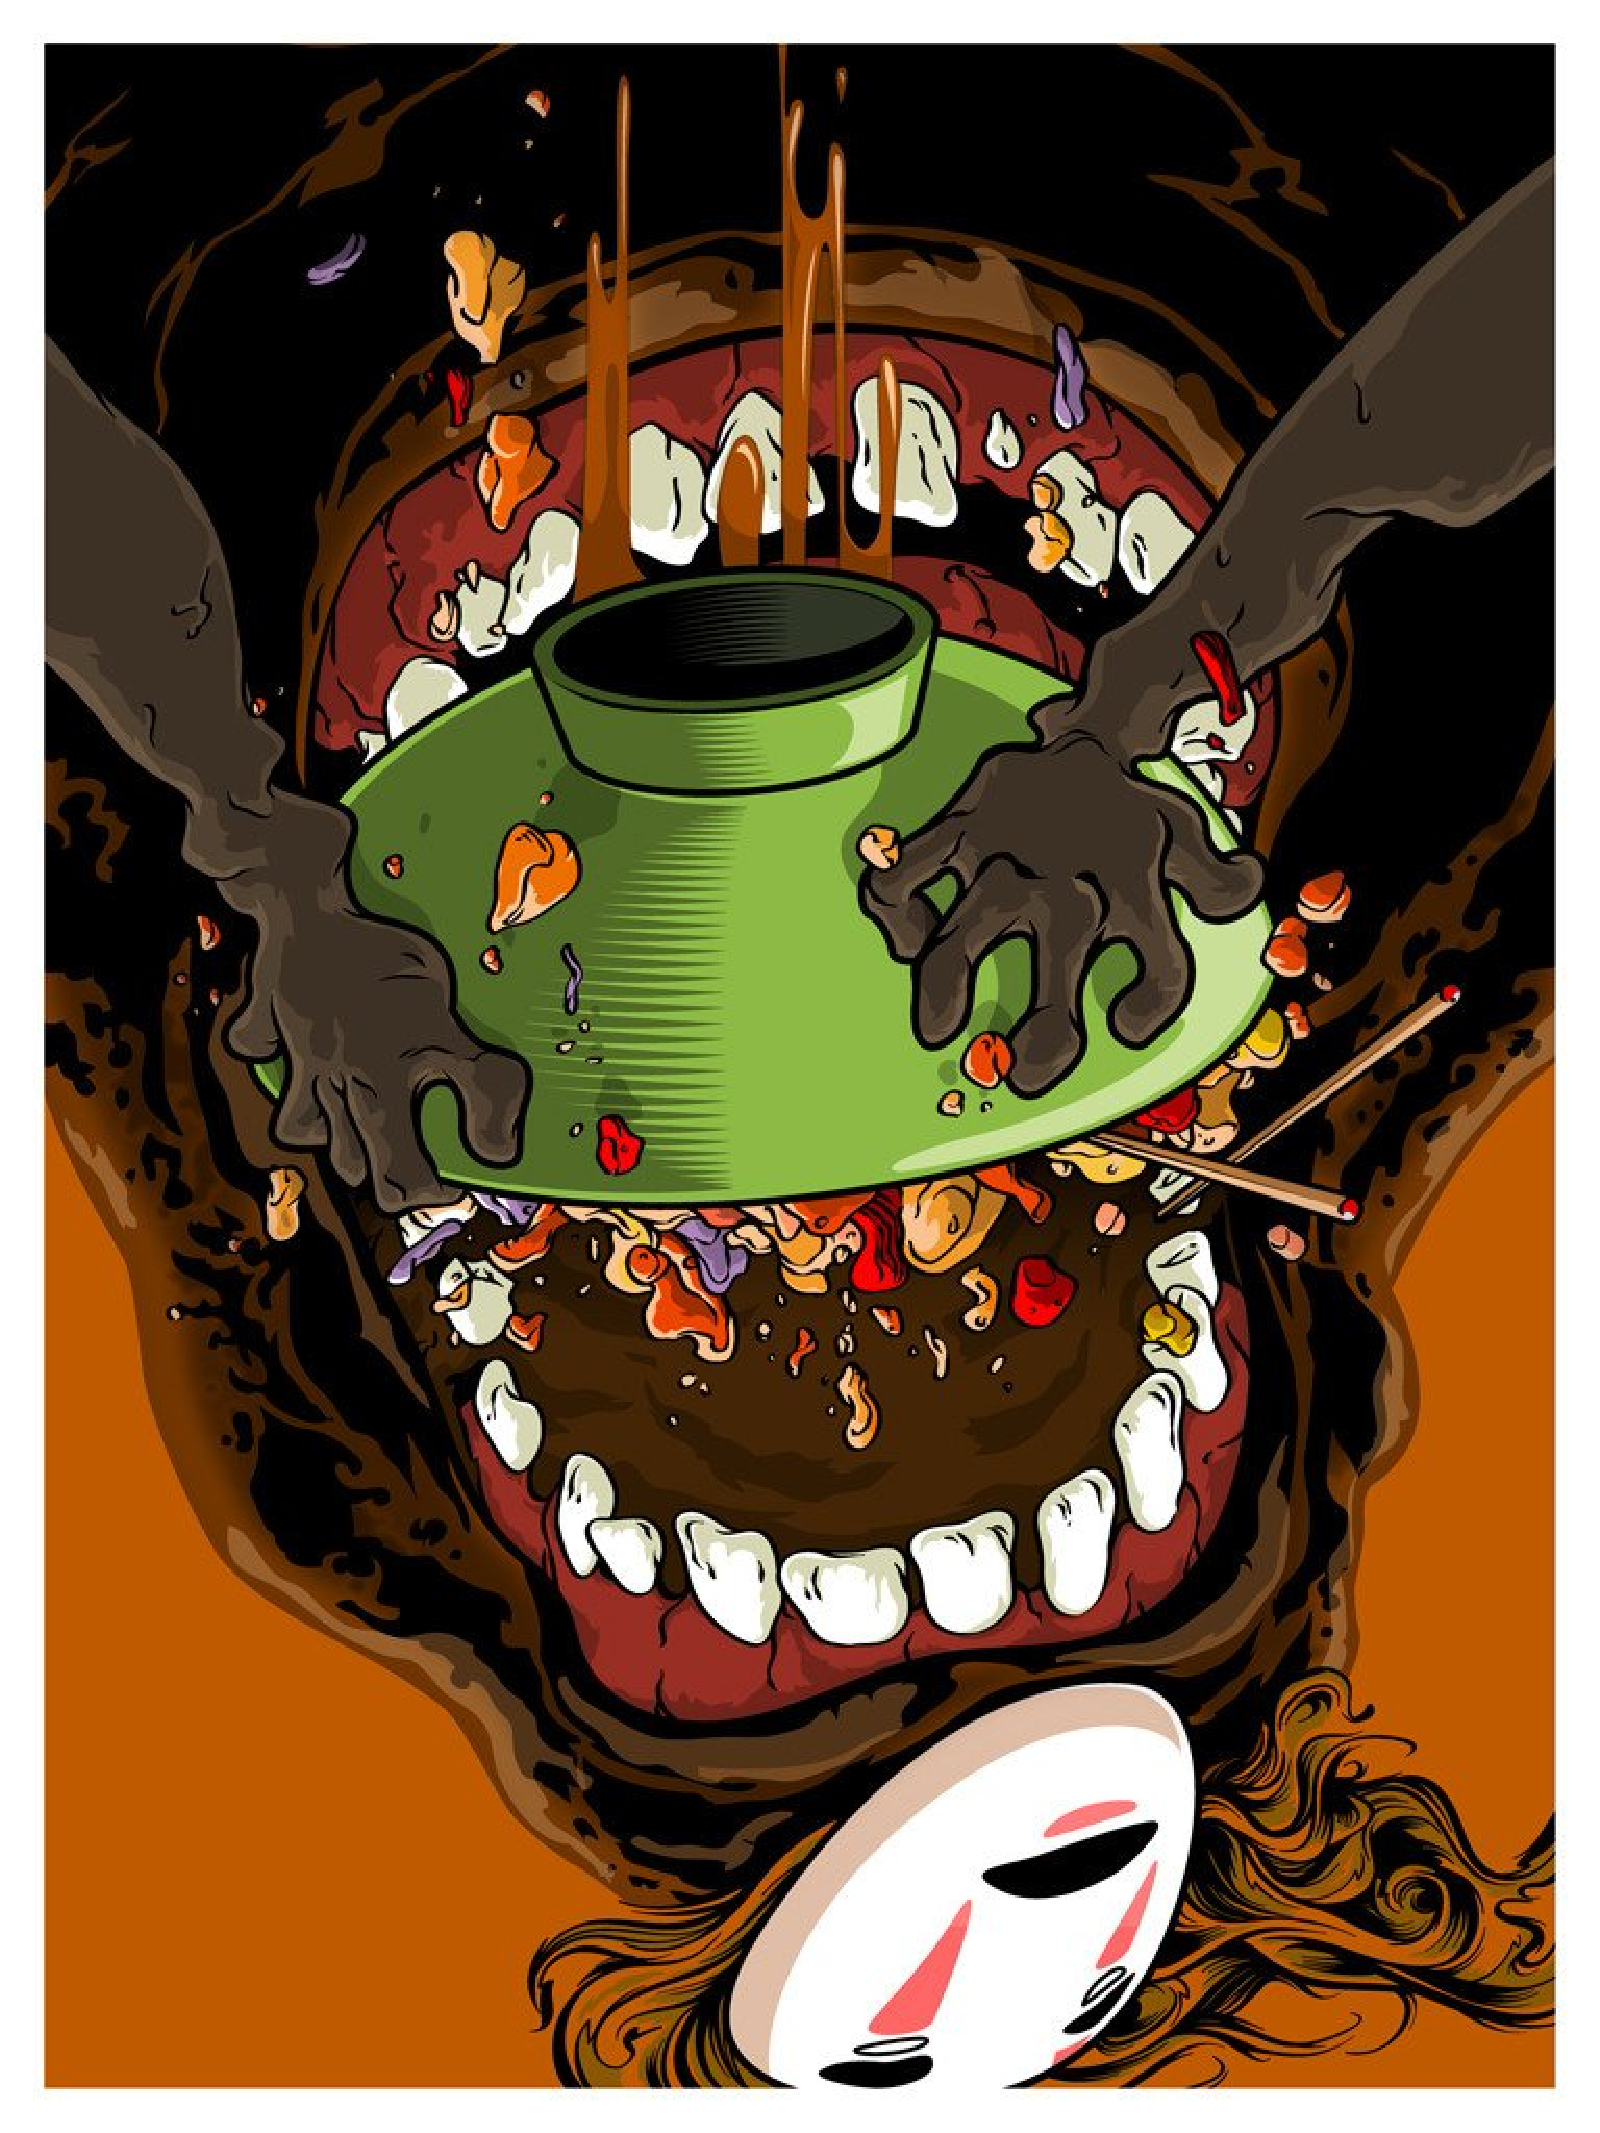
\includegraphics[height=6cm, width=5cm]{pop6.pdf}
	\end{turn}
	\end{minipage}
\end{figure}

\begin{figure}[h!]

	\begin{minipage}[h!]{0.3\linewidth} 
		\begin{turn}{180}
			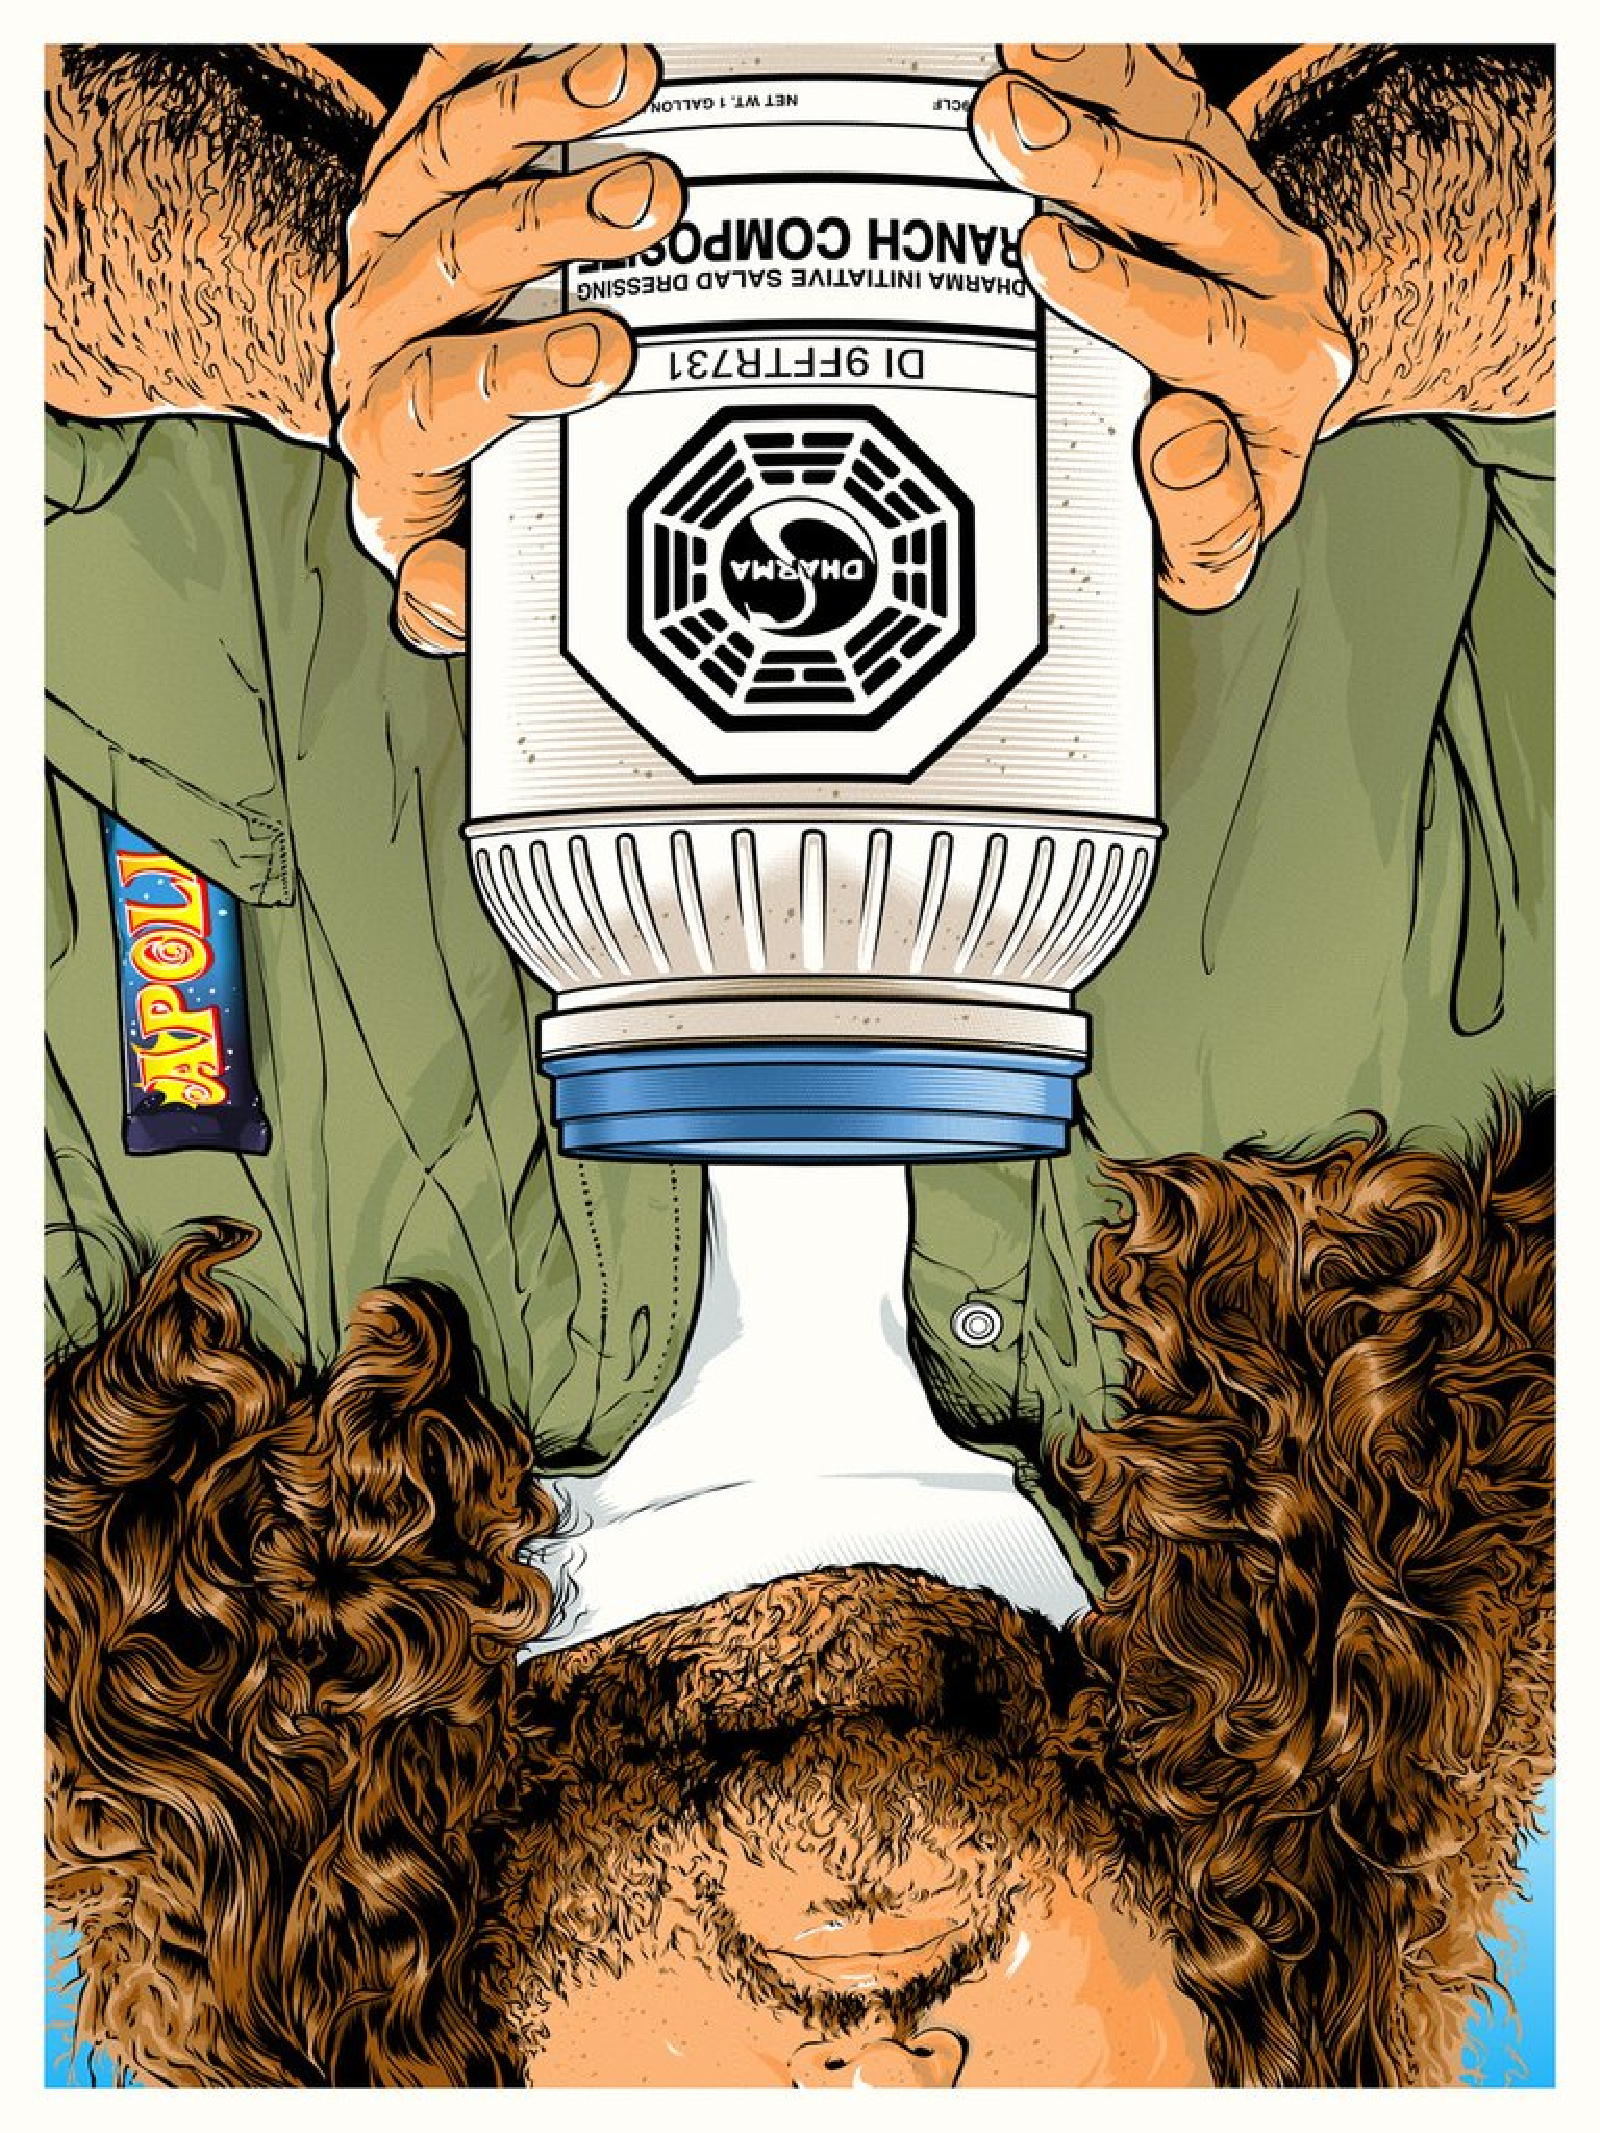
\includegraphics[height=6cm, width=5cm]{pop10.pdf}
		\end{turn}
	\end{minipage}
	\hfill
	\begin{minipage}[h!]{0.3\linewidth}
		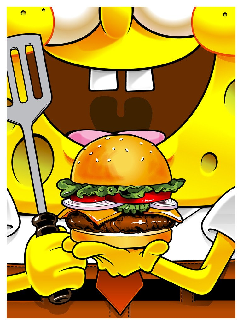
\includegraphics[height=6cm, width=5cm]{pop8.pdf}
	\end{minipage}
    \hfill
	\begin{minipage}[h!]{0.3\linewidth} 
		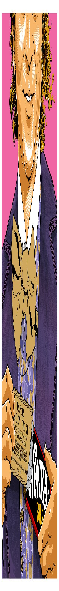
\includegraphics[height=6cm, width=5cm]{pop7.pdf}
	\end{minipage}
\end{figure}

\end{document}